%!TEX root = ../my_thesis.tex
\chapter{Processeurs personnalisés à faible consommation pour le décodage SC} % (fold)
\label{chap:tensilica}

\vspace*{\fill}
\minitocTITI
\vspace*{\fill}
\newpage

\section*{Introduction}
Les implémentations logicielles des fonctions de traitement du signal dans les infrastructures de communication radio sont encouragées pour tendre vers un réseau virtualisé de type Cloud-RAN. De telles implémentations sont présentées pour les algorithmes de décodage polaire à liste dans le chapitre précédent. De hauts débits peuvent être atteints, et la flexibilité et la généricité de ces décodeurs est très importante. En utilisant des processeurs visant des systèmes électroniques embarqués, ces implémentations peuvent également gagner en efficacité énergétique.

Toutefois, les processeurs à usage général incluent de nombreuses unités matérielles destinées à réaliser efficacement de nombreuses et diverses applications. Mais ces unités matérielles ne sont pas utilisées dans certaines de ces applications. Par exemple, dans les algorithmes de décodage de canal, toutes les unités de calcul à point flottant sont inutiles puisqu'une représentation des données interne par virgule fixe est suffisante. Ces unités matérielles consomment de l'énergie inutilement. Le profilage d'un décodeur polaire montre que la majeure partie du temps d'exécution est passé à réaliser un ensemble restreint de fonctions élémentaires. De plus, une part significative des instructions exécutées correspond à des opérations de sauvegarde et de chargement de données dans les registres.

Ces observations poussent à envisager la conception d'un processeur programmable qui exclurait les unités matérielles inutiles des processeurs à usage général, tout en intégrant des unités de calculs spécialisées dans la réalisation efficace des fonctions élémentaires de décodage de codes polaires. Ce type de processeurs entre dans la catégorie des processeurs à jeu d'instructions spécifique à l'application (ASIP: Application Specific Instruction-set Processor).

Les Chapitres \ref{chap:tensilica} et \ref{chap:tta} de ce manuscrit présentent deux architectures de processeurs ASIP spécialisées pour le décodage de code polaire. Ces deux architectures ont été conçues selon des méthodologies de conception différentes. Dans la Section \ref{sec:asips}, le concept d'ASIP est introduit, et la méthodologie utilisé pour la première architecture est décrite. Dans la Section \ref{tensilica_design}, la conception de l'ASIP est détaillée. Enfin les résultats d'implémentation et les performances de l'architecture en termes de débit, latence, complexité et consommation énergétiques sont présentés et discutés.


\section{Les processeurs à jeu d'instructions spécifiques à l'application}
\label{sec:asips}

\subsection{Définir un ASIP}
Un ASIP est une architecture programmable permettant la description logicielle d'un algorithme et possédant des unités matérielles spécifiques à une application.
\subsection{Langages de description matérielle}
\subsection{ASIP au sens de Tensilica}

Le jeu d'instructions (ISA : )
- Configurabilité et extensivité


\section{Conception d'un ASIP Tensilica pour le décodage de codes polaires}
\label{tensilica_design}

\subsection{Implémentations matérielles de l'algorithme SC}
\label{subsec:sota_sc}
\subsection{Configuration}
\subsubsection{Architecture de base}
La philosophie de conception de l'ASIP proposé est de réaliser l'ensemble des fonctions élémentaires polaires à l'aide d'unités matérielles spécialisées, tandis que les opérations de contrôle sont effectuées par les unités matérielles de base du processeur XTensa. Ce processeur de base est donc dépourvu de tout accélérateur matériel optionnel. Il n'y a pas d'unité de calcul flottant, d'unité MAC (Multiple and Accumulate) ou d'unité accélérant les divisions.

Par contre, la fonctionnalité FLIX () de Tensilica correspond à la possibilité d'ajouter des pipelines d'exécution dans l'ALU principale. Cela permet au processeur d'exécuter plusieurs instructions en parallèle. Il est possible de configurer les instructions réalisées par chaque pipeline. Notre choix s'est porté sur une configuration nommée FLIX3 prédéfinie par l'outil de conception. Ainsi, trois instructions faisant partie du jeu d'instruction de base peuvent être appliquées sur trois données de 32 bits simultanément. Ce parallélisme d'instruction permet de réaliser plus rapidement les fonctions de contrôle et de calcul d'adresse. 

\subsubsection{Quantification des données}
Il est démontré dans \cite{sarkis_fast_2014} que des LLRs représentés sur 6 bits permettent d'égaler les performances de décodage d'implémentations en virgule flottante. Cependant, il est plus simple dans une implémentation logicielle de représenter ces données sur 8 bits puisque les langages de programmation définisse de tels types de données. Comme montré dans \cite{leroux_hardware_2011}, à un niveau $d$ de l'arbre de décodage doivent être stockés $2^{n-d}$ LLRs. La taille de la mémoire permettant de stocker les LLRs est donc de $2^{n+1}-1$ octets.

Les sommes partielles sont des valeurs binaires. Cependant, encore une fois, la manipulation des sommes partielles dans le langage de description logicielle est plus aisée si l'on utilise un entier de 8 bits pour représenter chaque somme partielle. Il serait cependant possible d'utiliser un entier pour représenter 8 sommes partielles, ce qui réduirait l'empreinte mémoire de celles-ci. Cela nécessiterait cependant des opérations de masquage supplémentaires et plus d'irrégularités dans les accès aux données.

\subsubsection{Configuration de la mémoire cache}
Le choix a été fait d'augmenter au maximum le parallélisme des instructions élémentaires nécessaires au décodage de codes polaires. La taille maximum des registres du processeur XTensa, qui est donc la taille utilisée dans l'ASIP proposé, est de 512 bits. Afin de pouvoir charger et sauvegarder des données depuis et vers la mémoire cache en un seul cycle d'horloge, la largeur d'une ligne de mémoire cache est également de 512 bits. La taille de ces mémoires ainsi que leur associativité est également configurable. Des expérimentations ont été réalisées afin de sélectionner ces valeurs. Dans tous les cas testés, un associativité à 4 voies pour les mémoires d'instructions et de données est permet les meilleures performances.

En ce qui concerne la taille de la cache, bien que le plus petit nombre d'échec d'accès à la mémoire cache soit atteint pour la taille de cache la plus grande (128 kilooctets), une mémoire d'instruction de 8 kilooctets ainsi qu'une mémoire de données de 8 kilooctets est suffisante pour atteindre un nombre d'échecs de cache seulement 5 \%
plus grand que la valeur optimale.

\subsection{Instructions spécialisées}
\begin{figure}[t]
  \centering
  \subfloat[Fonction $f$]{
  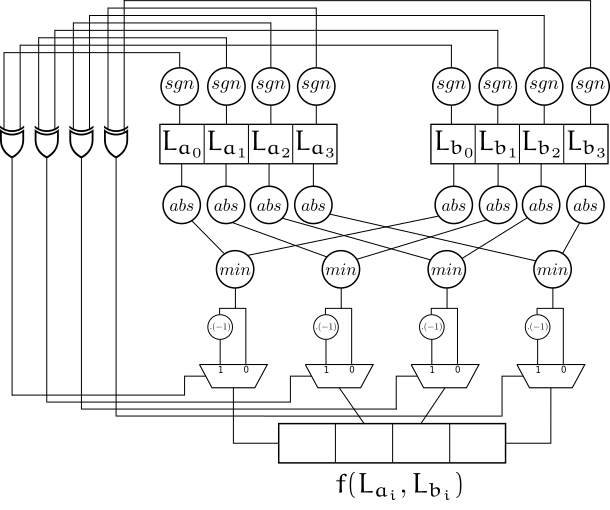
\includegraphics[scale=0.45]{main/ch3_fig/f_tie}
  \label{fig:f_tie}
  }
  \subfloat[Fonction $g$]{
  \includegraphics[scale=0.45]{main/ch3_fig/g_tie}
  \label{fig:g_tie}
  }
  \caption{Unités matérielles des fonctions $f$ et $g$}
\end{figure}
La conception des instructions spécialisées est basée sur les unités matérielles décrites dans la littérature des implémentations matérielles de l'algorithme SC décrites en Section \ref{subsec:sota_sc}. Ces instructions spécialisées sont donc décrites à l'aide du langage TIE de Tensilica.
L'implémentation de la fonction $f$ est représentée dans la Figure~\ref{f_tie}. Les deux entrées sont les LLRs notés $L_a$ et $L_b$ et la sortie est notée $f(L_a,L_b)$. Souvent, pour réduire le chemin critique, les LLRs sont représentés en \og signe-amplitude \fg : un bit est utilisé pour le signe, et le reste pour la valeur absolue, toujours positive. Dans notre implémentation, les valeurs négatives sont représentées en complément à deux, car il s'agit du mode de représentation utilisé dans les processeurs XTensa.
La fonction $g$ est représentée dans la Figure~\ref{g_tie}. Elle consiste en une addition simple avec une inversion de signe selon la valeur de la somme partielle $s_a$.
La fonction $h$ n'est pas représentée, il s'agit simplement d'un ou-exclusif entre les sommes partielles d'entrées. Les fonctions \texttt{R0} et \texttt{R1} sont également très simples est leur représentation graphique n'est pas utile, puisqu'il s'agit d'une mise à zéro dans le premier cas, et d'un seuillage dans le deuxième, c'est à dire une simple copie du bit de poids fort.

Comme présenté dans la Section~\ref{subsec:pruning}, le traitement d'un \noeud de répétition consiste en l'addition de tous les LLRs d'entrée pour former la variable notée \og \texttt{accum} \fg dans la Figure~\ref{fig:rep_tie}. Puis de la détection du signe de cette variable, qui détermine le vecteur $s$ en sortie. Un arbre binaire est parcouru afin de réaliser l'addition nécessaire. Pour éviter tout débordement, la taille du registre de stockage de la variable \texttt{accum} est de 32 bits.

L'unité matérielle de traitement des \noeuds \texttt{SPC} est représentée dans la Figure~\ref{fig:spc_tie}


\subsection{Description logicielle}
Lors du développement, il est apparu qu'il était difficile de réduire le temps passé à réaliser les opérations liées au parcours de l'arbre et aux différents tests. L'utilisation de l'option FLIX3 a permis de réduire ce temps, mais pas suffisamment. La technique de déroulage présentée en Section~\ref{subsec:unroll} permet de réduire ce temps. Dérouler le code signifie sacrifier en flexibilité. En effet, il faut générer une version différente du code pour un ensemble donné de paramètres.

Une alternative est utilisée dans l'implémentation proposée. Tout d'abord, toutes les fonctions élémentaires pour le décodage de code polaires possèdent le même prototype de fonctions dans la description logicielle. Le type de fonction à appliquer ($f$, $g$, $h$, \texttt{R0}, \texttt{R1}, \texttt{SPC}, \texttt{REP}) est passé en paramètre de la fonction, accompagné des adresses auxquelles accéder aux données à lire et écrire. De cette manière, il est possible de créer, un tableau contenant les pointeurs des fonctions à appeler. L'algorithme permettant de déterminer la séquence de fonctions à exécuter prend comme entrée le tableau de bits gelés correspondant au code polaire traité.


\section{Expérimentations et mesures}

\subsection{Estimation de complexité}
\subsection{Comparaisons}

\section*{Conclusion}

